\ifgerman{\chapter{Vorgeschlagene Methoden}}{\chapter{Modeling performance estimation as a learning process}}
\label{methods}
As described in the previous section, current performance estimation methods can be roughly categorized into two sections. One group uses information present for the current state of a classifier, e.g. the cross-validation methods. The second, much smaller group takes a look at the performance development over time, up to the current iteration. This encompasses the fitting of function models expected to be of similar shape to the learning curve using already present performance estimates to extrapolate them to future iterations. Typical methods for the estimation of the already witnessed iterations include holdout testing and k-fold cross-validation \cite{FigueroaEtal2012}.

The methods proposed in this work focus on combining both groups in an attempt to use as much information as possible to increase the prediction quality; .632 bootstrapping and the likes focus on the set of available instances, ignoring the process that led to this state. In turn, curve fitting currently makes use of either subpar techniques to obtain the accuracies for each iteration or uses holdout samples which can be costly or not available at all.

To serve as an illustration of the thought process leading to the following techniques, we assume, without loss of generality, a dataset $D = {(\vec{x_i}, y_i)}$ with two class labels $y_i \in {0, 1}$ and $|D| = n$. From this set an active learner selects $k \leq n$ instances which serve as the training set $X_T$ of a classifier $c: \vec{x} \mapsto y$. We would like to know the prediction accuracy of $c$ for the set $D$.

\section{Performance estimation on training sub-sets}
The simplest way to obtain performances estimates for the process of instance selection would be to use \textit{leave-x-out(LXO) cross-validation}, with $x \in \{1,...,k-1\}$. This way, we obtain $k \choose x$ subsets $S_{T,i}$ of size $x$ from the original training set as well as corresponding test sets of size $k-x$, which enable the performance estimation. Both low computational cost for the individual estimates as well as unbiasedness \cite{RodriguezEtAl2013} make it a reasonable choice. While the computational effort for each subset is low, the total amount of possible subsets is $2^k - 2$, only leaving out the edge cases with size 0 and $k$, resulting in exponential complexity if used natively. Thus, some kind of sampling to reduce the complexity seems desirable.

Another option with regard to the estimation is \textit{bootstrapping}. It offers a little more variety, as different types like \textit{na\"{i}ve}, \textit{leave-one-out} and \textit{.632} are available. This comes at a price, however; additional computational effort for the creation and testing of the bootstrap samples is necessary. Also, it isn't trivial how to create and handle the subsets. One could proceed similar to its cross-validation counterpart, sampling from the training set without replacement and using that subset as base for the bootstrap samples. This has two obvious downsides: for one, we are unable to obtain performance estimates for set sizes of one (except for na\"{i}ve bootstrap, which doesn't require that test instances are not within the bootstrap sample). To solve this, the instances not selected for the subset could be used as (additional) test sets, as they are when using cross-validation. However, the influence this would have on the .632 family is unclear; although theoretically additional test instances should not revoke the name-giving necessity of weighting between training and bootstrap performance, the weights themselves may be incorrect, as the bootstrap would be tested on data not available to the training performance estimation. Of course, a possibility could be to also test the training performance on those additional instances, but then it wouldn't be the training error anymore, making it even more unclear.

\subsection{Sub-sampling of fitting points}
Regardless of which estimation technique is used, the complexity still scales exponentially with the set size $k$. To reduce the amount of estimates for the fitting process, some sort of selection has to occur. In this work, three sub-sampling strategies were explored. Reducing the information available naturally has some drawbacks, including an expected higher variance and, if done improper, an added bias. Also, the sampling may influence the fitting itself, potentially inflicting additional penalties to the robustness.

A simple, yet effective method is to cap the number of estimates. Possible options are to either impose a fixed, hard cap for all training set sizes $|X_T|$, or to use a polynomial dependent on $k$, e.g. $k^2$. A potential pitfall is the selection of the subsets $S_{T,i} \subset X_T$ to be evaluated. Selecting either randomly over all possible subsets or from pools for each subset size $|S_{T,i}| \in \{1,...,k-1\}$ with sizes proportional to $|S_{T,i}| \choose k$ prevents unintentional importance assignment to subset sizes.

A related approach exports the computational cost to the fitting process. Instead of selecting multiple subsets per size once and using them for fitting, we select only one subset per size multiple times and fit on them separately. Formally, we have a tuple $\tilde{S_j} = (S_1,...,S_{k-1})$ with $S_i \subset X_T$, $|S_i| = i$ and $j = \{1,...,r\}$. The $S_j$ can be drawn with or without replacement, although the latter may lead to a lower variance, as seeing the same constellation multiple times does not add information, whereas a different one does. The parameter $r$ is up to choosing, with an upper limit of $\prod_{i=1}^{k-1} {k \choose i}$ as the number of combinations for drawing without replacement. This would result in a higher complexity than exponential, namely $O(k!)$. However, accounting for all possible subset combinations may not be necessary, as there are far less unique combinations of accuracy estimations. This is due to the number of test instances available for a given training subset. For example, a classifier trained on a set of size one tested against a set of size three will have four potential test outcomes: either one, two, three or none instances were correctly classified, resulting in an estimated accuracy of $\frac{1}{3}, \frac{2}{3}, 1$ and $0$, respectively. As a grow in size of the training set in turn causes a reduction in size of the test set, the amount of potential outcomes shrinks from $k$ to $2$ for $|S_T| = \{1, ..., k-1\}$. Thus, the number of unique combinations would shrink to $k!$.

\begin{figure}[h]
	\centering
	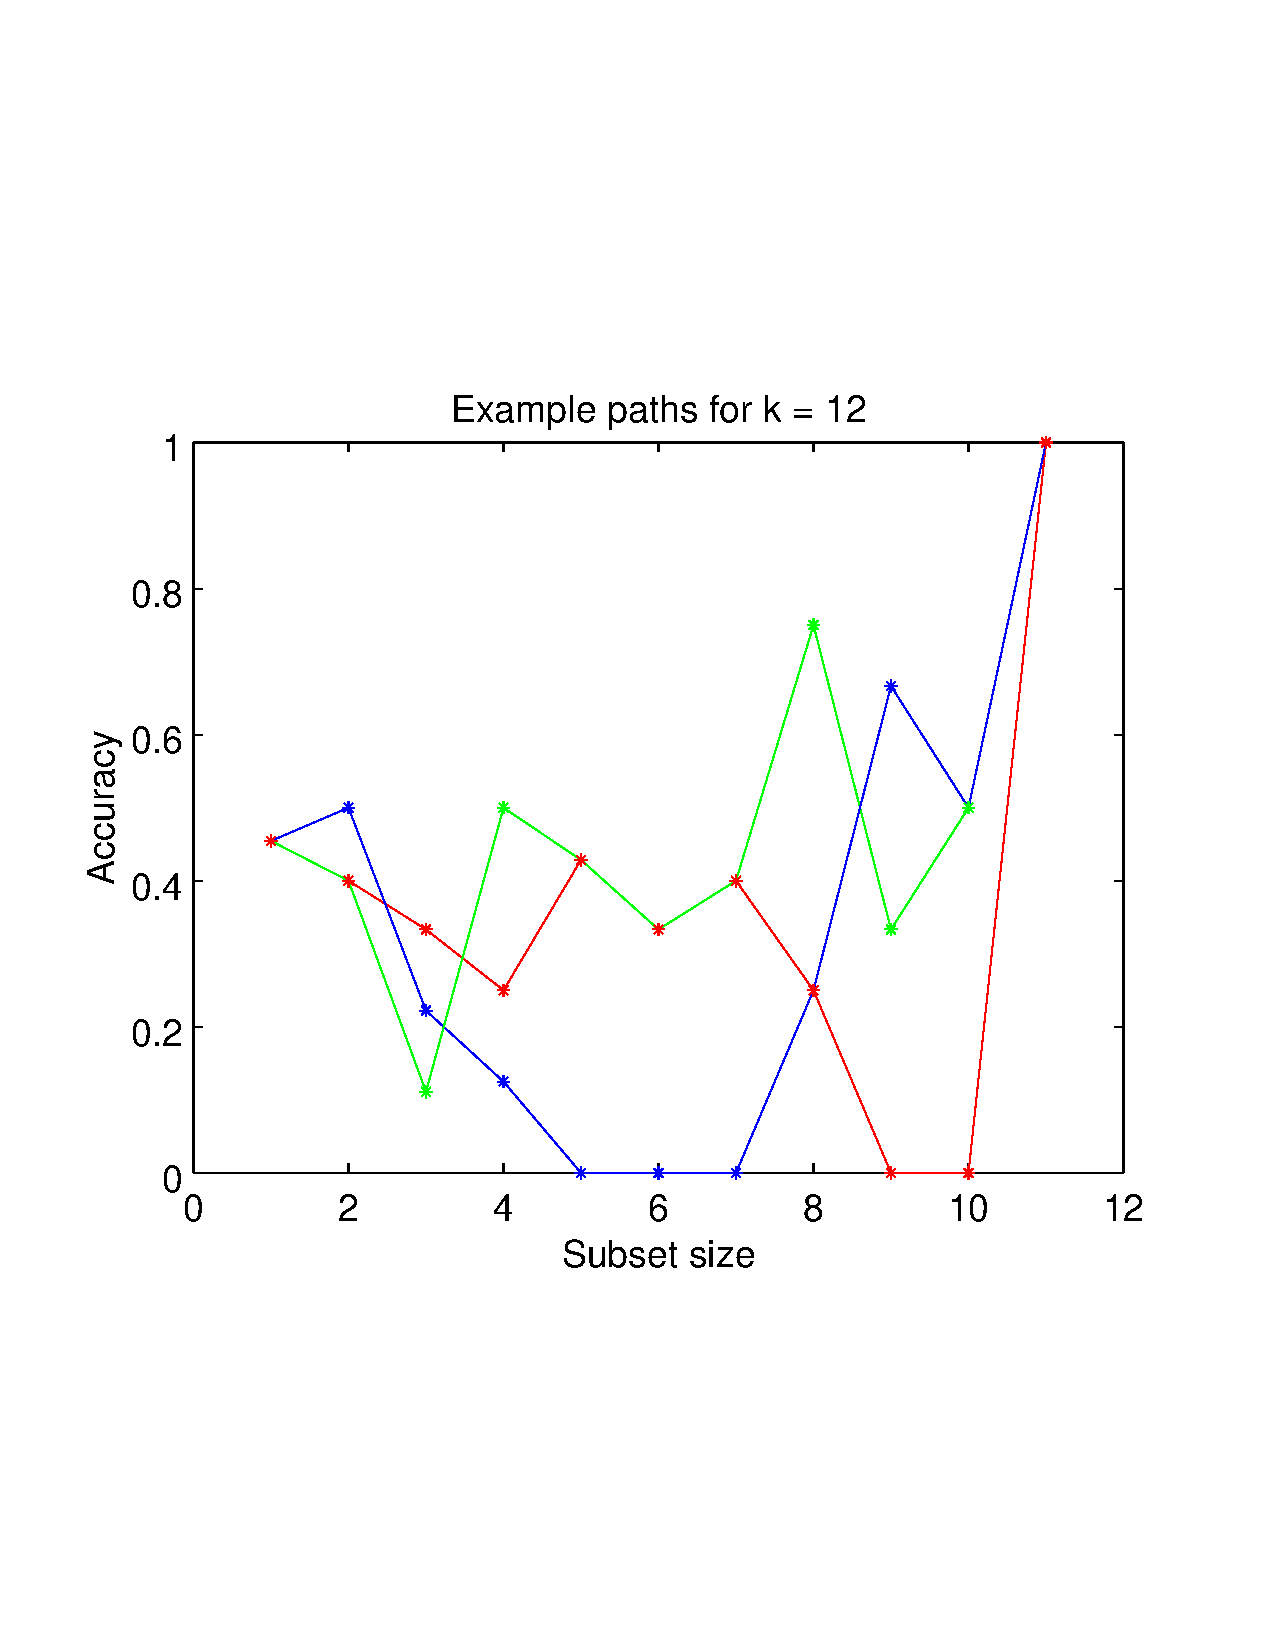
\includegraphics[trim = 0cm 6cm 0cm 5cm, clip = true, width = 0.45\textwidth]{pathExample1}
	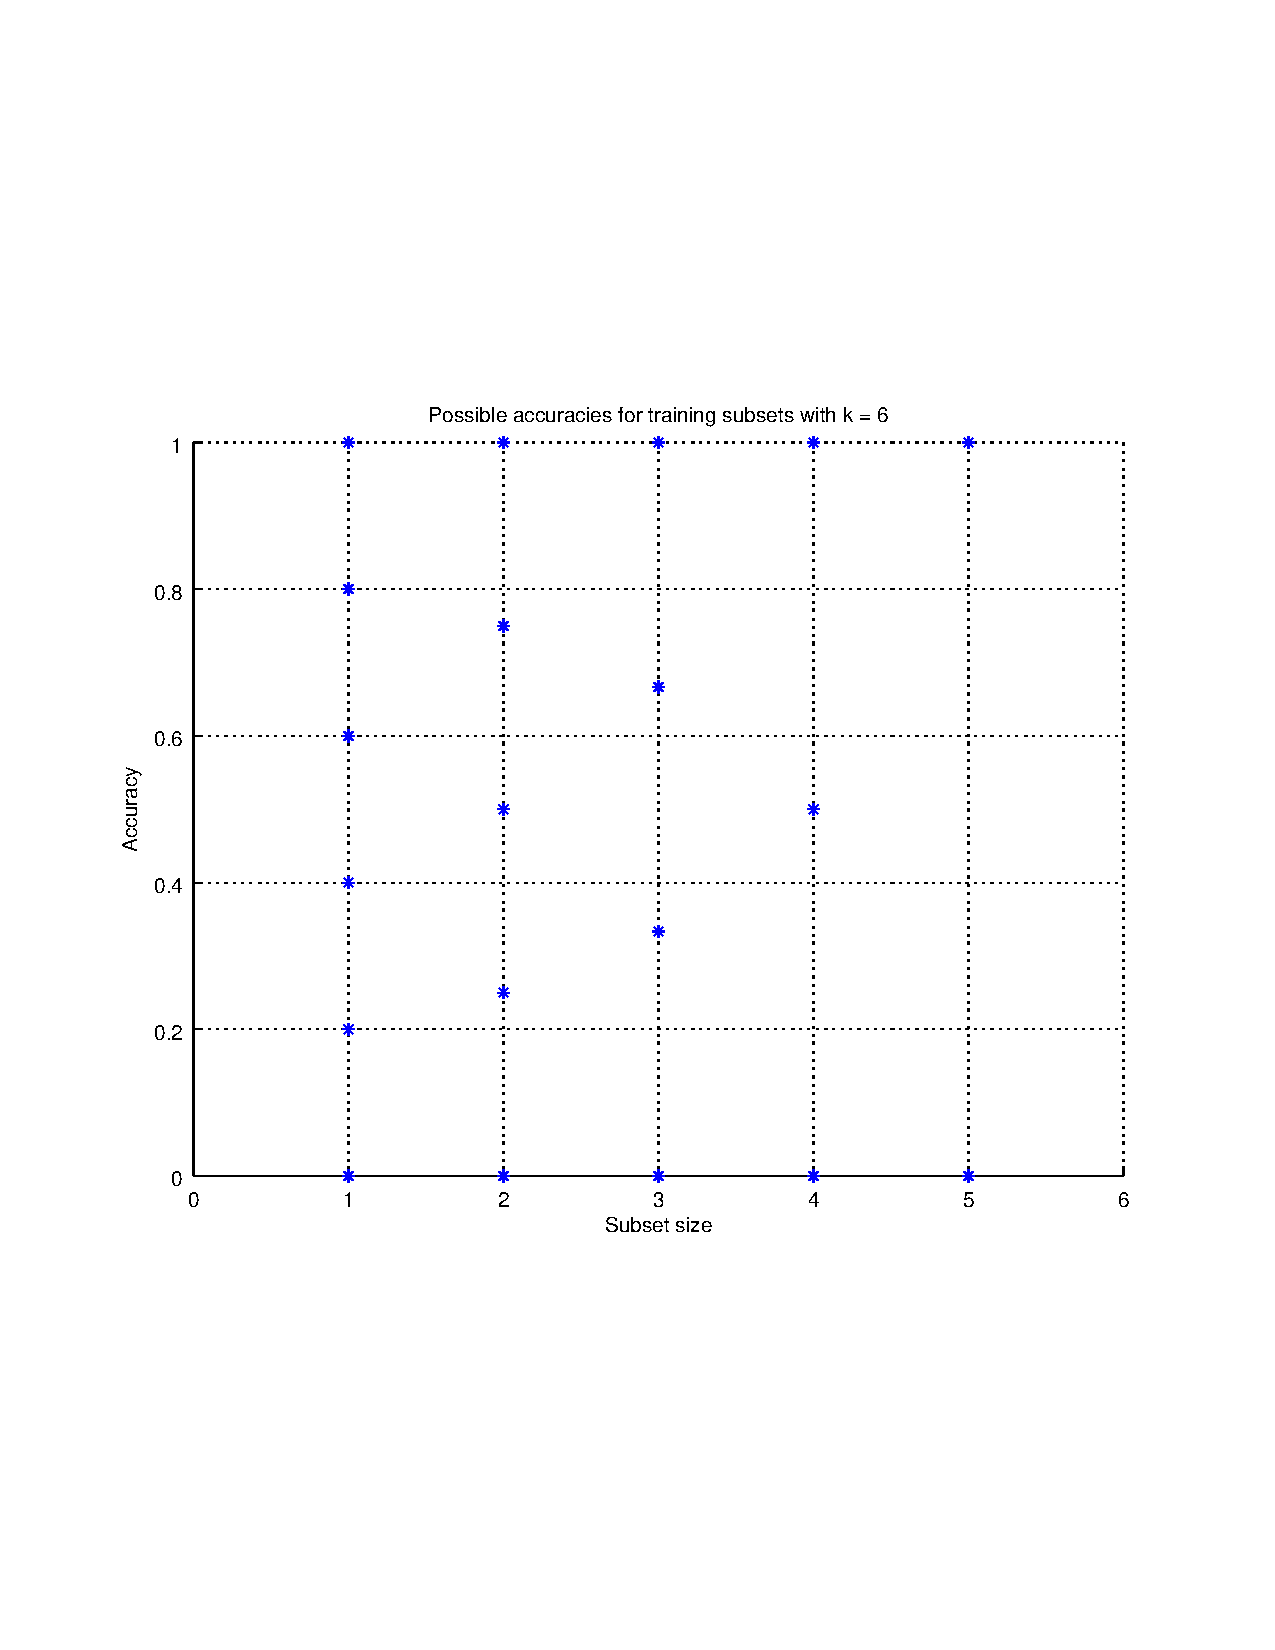
\includegraphics[trim = 0cm 6cm 0cm 5cm, clip = true, width = 0.45\textwidth]{accDemonstration}
	\caption{Left: Three example paths with superset restriction. The zigzag shape illustrates the difficulties for the fitting. Right: All possible accuracies for training subsets with $k = 6$}
	\label{fig:pathAccExamples}
\end{figure}

Unfortunately, in order to use the estimations as fitting data, they would have to be computed first; we need to know the distribution of accuracies for each subset size to weight them properly. Otherwise, a uniform weighting (or randomly picking one) would simply lead to a prediction of 0.5 and we would gain nothing. Thus, using the estimates themselves is not feasible as a reduction of estimation samples, but still limits the number of curves that have to be fit, as duplicates do not have to be fit twice; counting it twice for the final estimation suffices.

Taking a second look at the aforementioned method, something seems to be odd. As it is, randomly taking subsets of each size allows for something counterintuitive to happen: instances present in subsets of smaller size do not necessarily have to be selected for their larger brethren. However, a classifier trained by an active learner does not usually discard previously selected instances. Thus, it seems logical to restrict subsets of larger size to be supersets of their predecessors. This again reduces the possible combinations to $k!$, as the sampling is now done without replacement. This time, however, we do not rely on the final accuracy distribution, as each path is equally likely, meaning that the sub-sampling is applicable even without precomputing the estimates. This assumption only holds in general for random sampling; other active learners may show preferences for some instances which, in their eyes, improves the classifier's performance the most.

\begin{algorithm}
	\begin{algorithmic}[1]
		\State {$X_T = \left\{\vec{x}_1,...,\vec{x}_k\right\}$}
		\Comment {Current training set}
		\State {}
		\State {$subsets \gets powerset(X_T)$}
		\Comment {Compute all possible subsets}
		\State {$subsets \gets listBySize(subsets)$}
		\Comment {Categorize the subsets by size}
		\State {}
		\State {$samples \gets \{\}$}
		\For {$i \gets 1$ $to$ $|X_T|-1$}
		\State {$numOfSamples \gets \frac{1}{SAMPLE\_CAP} \cdot {|X_T| \choose i}$}
		\For {$j \gets 1$ $to$ $numOfSamples$}
		\State {$currSample \gets drawWithoutReplacement(subsets[i])$}
		\Comment {Get a random subset of size i and remove it}
		\State {$samples \gets {samples, currSample}$}
		\EndFor
		\EndFor
	\end{algorithmic}
	\caption{Capped sub-sampling}
	\label{alg:cappedSubSampling}
\end{algorithm}

\begin{algorithm}
	\begin{algorithmic}[1]
		\State {$X_T = \left\{\vec{x}_1,...,\vec{x}_k\right\}$}
		\Comment {Current training set}
		\State {}
		\State {$subsets \gets powerset(X_T)$}
		\Comment {Compute all possible subsets}
		\State {$subsets \gets listBySize(subsets)$}
		\Comment {Categorize the subsets by size}
		\State {}
		\State {$paths \gets \{\}$}
		\For {$i \gets 1$ $to$ $NUM\_OF\_PATHS$}
		\State {$currPath \gets \{\}$}
		\For {$j \gets 1$ $to$ $|X_T-1|$}
		\State {$currPath \gets \{currPath, drawRandom(subsets[j])\}$}
		\Comment {Get a random subset of size j}
		\EndFor
		\State {$paths \gets \{paths, currPath\}$}
		\EndFor
	\end{algorithmic}
	\caption{Unrestricted path sub-sampling}
	\label{alg:unresPathSubSampling}
\end{algorithm}

\begin{algorithm}
	\begin{algorithmic}[1]
		\State {$X_T = \left\{\vec{x}_1,...,\vec{x}_k\right\}$}
		\Comment {Current training set}
		\State {}
		\State {$subsets \gets powerset(X_T)$}
		\Comment {Compute all possible subsets}
		\State {$subsets \gets listBySize(subsets)$}
		\Comment {Categorize the subsets by size}
		\State {}
		\State {$paths \gets \{\}$}
		\For {$i \gets 1$ $to$ $NUM\_OF\_PATHS$}
		\State {$currPath \gets \{\}$}
		\For {$j \gets 1$ $to$ $|X_T-1|$}
		\State {$validSubsets \gets contains(subsets[j], currPath)$}
		\Comment {Limit the available subsets to supersets of the current path}
		\State {$currPath \gets \{currPath, drawRandom(validSubsets)\}$}
		\Comment {Get a random subset}
		\EndFor
		\State {$paths \gets \{paths, currPath\}$}
		\EndFor
	\end{algorithmic}
	\caption{Restricted path sub-sampling}
	\label{alg:resPathSubSampling}
\end{algorithm}

\subsection{Grouping of performance estimates}
Now that the subsets have been selected, the individual performances have to be estimated. For the cross-validation approach, this requires a classifier being trained on each of them and testing it on the remaining instances $X_T \setminus S_i$. Next in line is the decision which estimates to use for the fitting, and how. Depending on the sub-sampling selected, different options are available:

\begin{itemize}
	\item \textbf{All data}: The performance estimates are combined with their respective subset size and then used to fit a single curve.
	\item \textbf{Averaged data}: As originally intended for leave-x-out, the estimates are first arithmetically averaged over their respective subset size, then used to fit a single curve. This has the side effect that it skews the "importance" of the estimates, as more of them are available for middle-of-the-pack subset sizes. By not using all of them, the inherent weighting is removed.
	\item \textbf{One path at a time}: For the path-based sub-samplings, we only have one estimate per subset size anyway, but multiple times. Consequently, we fit one curve for each path. This results in multiple curves and thus multiple final performance estimates.
\end{itemize}

\section{Combining sub-estimates with curve fitting}

\subsection{Function models and fitting algorithms}
As a big part of the fitting process, some thought has to go into the selection of an appropriate function model. Not only does it have to be capable of modeling the learning process, it also largely determines the spectrum of algorithms available. For a linear model or one that can be linearized, e.g. the 2-parameter exponential law, the computation of the parameters which minimize the squared error is well known and trivial. More complex algorithms are necessary for functions which cannot be linearized, like the 3-parameter exponential law. Then, iterative methods have to be used, like the Levenberg-Marquardt algorithm \cite{Levenberg1944}. It works by iteratively adapting the parameters following its approximated gradient, with the goal to find a minimum for the least squares error function.

While they are able to handle a larger number of functions, they also need to be provided with various tuning parameters. In the case of Levenberg-Marquardt, initial values and maximal change per parameter as well as the partial derivatives w.r.t. the parameters must be given. Also, convergence is not guaranteed; unlike linear least squares, where minimizing parameters exist for at least two data points with different x components, poorly chosen initial parameters or too few iterations may lead to divergence. Potentially even more detrimental are local minima, as a divergence may be recognized. Here, the derivative of the error function is zero, indicating a minima, but different ones with lower absolute error values exist. However, the algorithm has no way of detecting this; the only options to avoid such a, quite literal, pitfall are to try the fitting with multiple initial parameters, hoping to get lucky, or to exploit previous knowledge about the data.

Potential function models were examined in section \ref{background}, especially in \cite{Singh2005}. A good candidate for least squares fitting seems to be the 3-parameter exponential law
\begin{equation}
f(x) = a + b \cdot e^(c \cdot x)
\end{equation}
Unfortunately, it falls in the category "non-linearizable" and requires iterative fitting. A different non-linearizable function class are sigmoids. For the evaluation, we also use a sigmoid of the form
\begin{equation}
f(x) = y_0 + 2 \cdot (y_0 - S) \cdot \left( \frac{1}{1+e^{m \cdot x}} - 0.5 \right)
\end{equation}
While they weren't tested in the cited articles, it can be similar in shape thanks to the exponential part and has the advantage of semantic parameters, that means they communicate the function's shape without the need to draw it. In this case, $y_0$ indicates the y-intercept, $S$ is the asymptotic threshold, and $m$ communicates the function's slope. This way, it is easier to find appropriate bounds for the parameters during fitting: clearly, a learning curve has to have both y-intercept and asymptote between 0 and 1 as well as a slope larger or equal to 0. While similar parameters can be found for the exponential function, they are not as precise, leaving more room for potentially wrong guessing, especially for the initial parameters.

Lastly, the fitted functions will be evaluated at the point $k$ using the parameters determined by the fitting. Since we potentially get more than one result as we may have multiple curves from the path sub-sampling, we then average the results to get a final performance estimate. The latter case also opens up the possibility of constructing a probability distribution, which will be discussed further in section \ref{evaluation}.

\subsection{Fitting improvements}
Usually, data gathered for curve fitting is not uniform, e.g. some data points are more likely to be tainted with error or do not carry much information. An example could be a study questioning people about the value of the elementary electric charge. Averaging the individual statements may, with a sufficiently large sample size, give an okay approximation to the real value. However, if the answers of people related to physics (students, engineers etc.) are counted twice, the approximation is likely to be better, as these people know generally more about physics and are thus more likely to know the correct answer.

To transfer this to our problem, we take a second look at the averaging grouping method. Here, we average the estimates and fit on them instead. This bears the problem of removing the information that for some fitting points more estimates were present. Using statistical weights in the fitting process proportional to the original amount of estimations brings this back into the fitting process, leading to correct importance of the data points. The influence on the fitting is depicted in \ref{fig:weigthingExample}.

\begin{figure}[h]
	\centering
	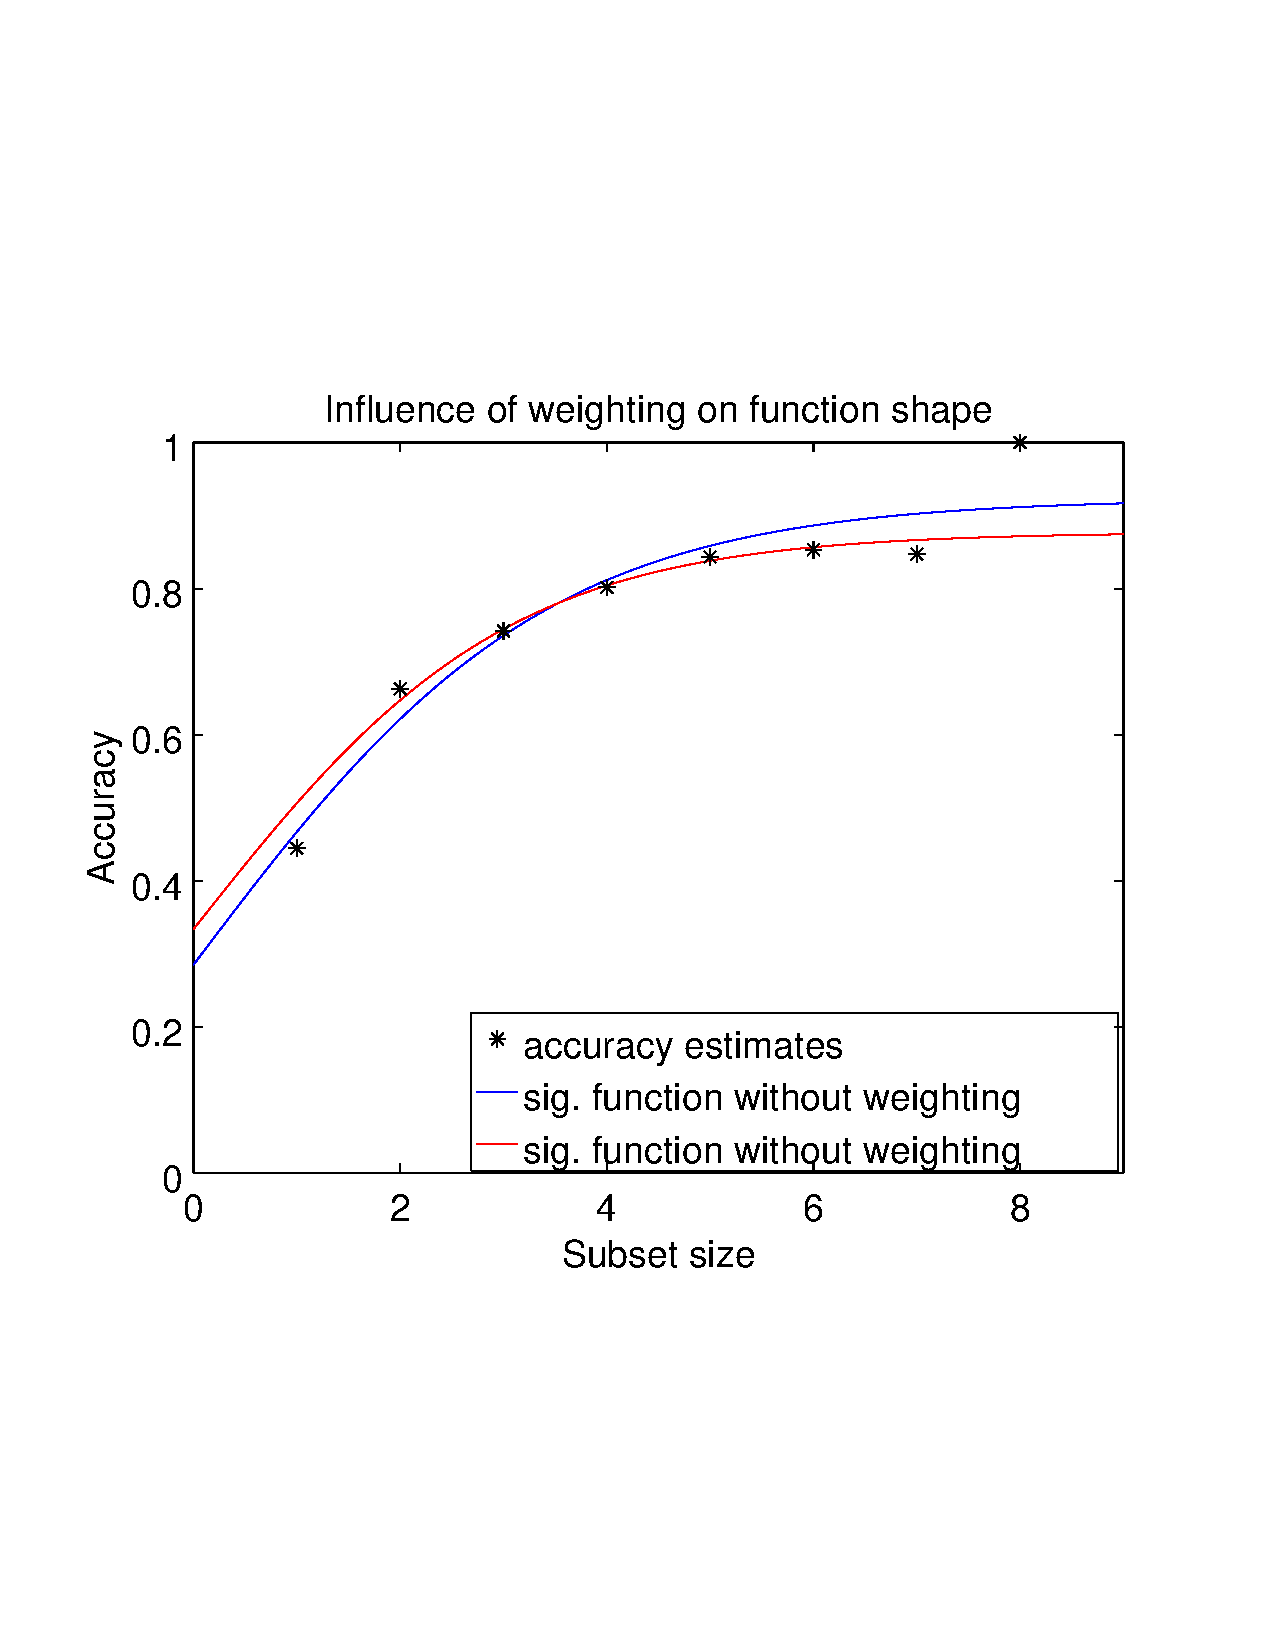
\includegraphics[trim = 0cm 6cm 0cm 5cm, clip = true, width = 0.7\textwidth]{weightingDiff}
	\caption{Difference between weighted and unweighted curve fitting for exponential functions The accuracies are not capped and averaged for $k = 10$}
	\label{fig:weigthingExample}
\end{figure}

Another potential improvement for the fitting process is the addition of data. Of course, while using the subset method, we cannot simply get more data without purchasing more labels. But we can get information for something that isn't covered by that method. Showcased in \cite{EfronEtAl1997} .632+ bootstrapping uses the \textit{no-information rate} to identify special overfit cases with data independent of its predictors. It is a heuristic used to approximate the error a classifier without any training would make when being tested on the dataset, the formula can be found in \eqref{eq:niRate}. And while we do have performance estimates for each subset size $|S_T| \in \{1, ..., k-1\}$, we are missing an estimate for $|S_T| = 0$. The no-information rate may be used as the 0th fitting point, filling that gap and help primarily with low $k$. For larger training sets, its influence should decrease as more "normal" estimates are available.

